\documentclass{standalone}
\usepackage{tikz}
\usetikzlibrary{patterns, positioning}

\begin{document}
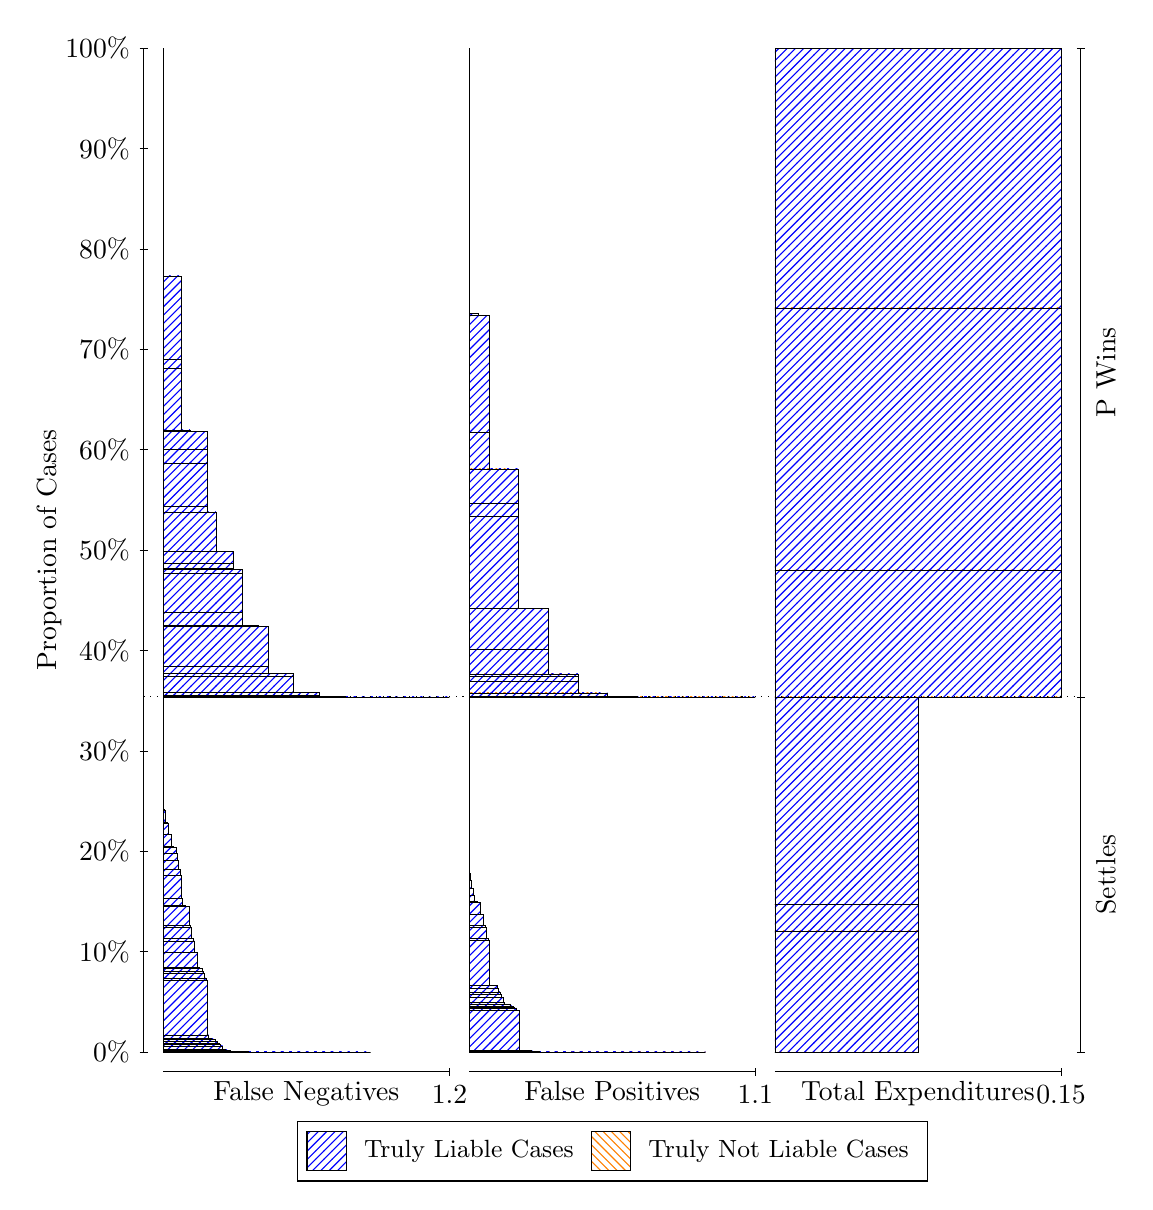
\begin{tikzpicture}
\draw[black, very thin] (1.5,1.75) -- (1.5,14.5);
\node[rotate=90, anchor=center] at (0.3, 8.125) {Proportion of Cases};
\draw[black, very thin] (1.45,1.75) -- (1.55,1.75);
\node[anchor=east] at (1.45, 1.75) {0\%};
\draw[black, very thin] (1.45,3.025) -- (1.55,3.025);
\node[anchor=east] at (1.45, 3.025) {10\%};
\draw[black, very thin] (1.45,4.3) -- (1.55,4.3);
\node[anchor=east] at (1.45, 4.3) {20\%};
\draw[black, very thin] (1.45,5.575) -- (1.55,5.575);
\node[anchor=east] at (1.45, 5.575) {30\%};
\draw[black, very thin] (1.45,6.85) -- (1.55,6.85);
\node[anchor=east] at (1.45, 6.85) {40\%};
\draw[black, very thin] (1.45,8.125) -- (1.55,8.125);
\node[anchor=east] at (1.45, 8.125) {50\%};
\draw[black, very thin] (1.45,9.4) -- (1.55,9.4);
\node[anchor=east] at (1.45, 9.4) {60\%};
\draw[black, very thin] (1.45,10.675) -- (1.55,10.675);
\node[anchor=east] at (1.45, 10.675) {70\%};
\draw[black, very thin] (1.45,11.95) -- (1.55,11.95);
\node[anchor=east] at (1.45, 11.95) {80\%};
\draw[black, very thin] (1.45,13.225) -- (1.55,13.225);
\node[anchor=east] at (1.45, 13.225) {90\%};
\draw[black, very thin] (1.45,14.5) -- (1.55,14.5);
\node[anchor=east] at (1.45, 14.5) {100\%};

\draw[black, very thin] (13.4,1.75) -- (13.4,14.5);
\draw[black, very thin] (13.35,1.75) -- (13.45,1.75);
\node[anchor=west] at (13.35, 1.75) {};
\draw[black, very thin] (13.35,6.2598) -- (13.45,6.2598);
\node[anchor=west] at (13.35, 6.2598) {};
\draw[black, very thin] (13.35,14.5) -- (13.45,14.5);
\node[anchor=west] at (13.35, 14.5) {};

\draw[black, very thin, pattern color=blue, pattern=north east lines] (1.75,1.75) rectangle (4.3823,1.75);
\draw[black, very thin, pattern color=blue, pattern=north east lines] (1.75,1.75) rectangle (4.234,1.75);
\draw[black, very thin, pattern color=blue, pattern=north east lines] (1.75,1.75) rectangle (4.0857,1.75);
\draw[black, very thin, pattern color=blue, pattern=north east lines] (1.75,1.75) rectangle (4.0528,1.75);
\draw[black, very thin, pattern color=blue, pattern=north east lines] (1.75,1.75) rectangle (3.9374,1.75);
\draw[black, very thin, pattern color=blue, pattern=north east lines] (1.75,1.75) rectangle (3.9045,1.75);
\draw[black, very thin, pattern color=blue, pattern=north east lines] (1.75,1.75) rectangle (3.7891,1.75);
\draw[black, very thin, pattern color=blue, pattern=north east lines] (1.75,1.75) rectangle (3.7562,1.75);
\draw[black, very thin, pattern color=blue, pattern=north east lines] (1.75,1.75) rectangle (3.7232,1.75);
\draw[black, very thin, pattern color=blue, pattern=north east lines] (1.75,1.75) rectangle (3.6408,1.75);
\draw[black, very thin, pattern color=blue, pattern=north east lines] (1.75,1.75) rectangle (3.6079,1.75);
\draw[black, very thin, pattern color=blue, pattern=north east lines] (1.75,1.75) rectangle (3.5749,1.75);
\draw[black, very thin, pattern color=blue, pattern=north east lines] (1.75,1.75) rectangle (3.4925,1.75);
\draw[black, very thin, pattern color=blue, pattern=north east lines] (1.75,1.75) rectangle (3.4596,1.75);
\draw[black, very thin, pattern color=blue, pattern=north east lines] (1.75,1.75) rectangle (3.4266,1.75);
\draw[black, very thin, pattern color=blue, pattern=north east lines] (1.75,1.75) rectangle (3.3937,1.75);
\draw[black, very thin, pattern color=blue, pattern=north east lines] (1.75,1.75) rectangle (3.3442,1.75);
\draw[black, very thin, pattern color=blue, pattern=north east lines] (1.75,1.75) rectangle (3.3113,1.75);
\draw[black, very thin, pattern color=blue, pattern=north east lines] (1.75,1.75) rectangle (3.2783,1.75);
\draw[black, very thin, pattern color=blue, pattern=north east lines] (1.75,1.75) rectangle (3.2454,1.75);
\draw[black, very thin, pattern color=blue, pattern=north east lines] (1.75,1.75) rectangle (3.1959,1.75);
\draw[black, very thin, pattern color=blue, pattern=north east lines] (1.75,1.75) rectangle (3.163,1.75);
\draw[black, very thin, pattern color=blue, pattern=north east lines] (1.75,1.75) rectangle (3.13,1.75);
\draw[black, very thin, pattern color=blue, pattern=north east lines] (1.75,1.75) rectangle (3.0971,1.75);
\draw[black, very thin, pattern color=blue, pattern=north east lines] (1.75,1.75) rectangle (3.0641,1.75);
\draw[black, very thin, pattern color=blue, pattern=north east lines] (1.75,1.75) rectangle (3.0476,1.75);
\draw[black, very thin, pattern color=blue, pattern=north east lines] (1.75,1.75) rectangle (3.0147,1.75);
\draw[black, very thin, pattern color=blue, pattern=north east lines] (1.75,1.75) rectangle (2.9817,1.7501);
\draw[black, very thin, pattern color=blue, pattern=north east lines] (1.75,1.7501) rectangle (2.9488,1.7501);
\draw[black, very thin, pattern color=blue, pattern=north east lines] (1.75,1.7501) rectangle (2.9158,1.7502);
\draw[black, very thin, pattern color=blue, pattern=north east lines] (1.75,1.7502) rectangle (2.8993,1.7502);
\draw[black, very thin, pattern color=blue, pattern=north east lines] (1.75,1.7502) rectangle (2.8664,1.7503);
\draw[black, very thin, pattern color=blue, pattern=north east lines] (1.75,1.7503) rectangle (2.8334,1.7526);
\draw[black, very thin, pattern color=blue, pattern=north east lines] (1.75,1.7526) rectangle (2.8005,1.7533);
\draw[black, very thin, pattern color=blue, pattern=north east lines] (1.75,1.7533) rectangle (2.7675,1.7538);
\draw[black, very thin, pattern color=blue, pattern=north east lines] (1.75,1.7538) rectangle (2.751,1.7539);
\draw[black, very thin, pattern color=blue, pattern=north east lines] (1.75,1.7539) rectangle (2.7345,1.7545);
\draw[black, very thin, pattern color=blue, pattern=north east lines] (1.75,1.7545) rectangle (2.7181,1.7546);
\draw[black, very thin, pattern color=blue, pattern=north east lines] (1.75,1.7546) rectangle (2.6851,1.7547);
\draw[black, very thin, pattern color=blue, pattern=north east lines] (1.75,1.7547) rectangle (2.6522,1.7595);
\draw[black, very thin, pattern color=blue, pattern=north east lines] (1.75,1.7595) rectangle (2.6192,1.7615);
\draw[black, very thin, pattern color=blue, pattern=north east lines] (1.75,1.7615) rectangle (2.6027,1.7712);
\draw[black, very thin, pattern color=blue, pattern=north east lines] (1.75,1.7712) rectangle (2.5862,1.7731);
\draw[black, very thin, pattern color=blue, pattern=north east lines] (1.75,1.7731) rectangle (2.5698,1.7752);
\draw[black, very thin, pattern color=blue, pattern=north east lines] (1.75,1.7752) rectangle (2.5368,1.7781);
\draw[black, very thin, pattern color=blue, pattern=north east lines] (1.75,1.7781) rectangle (2.5039,1.8264);
\draw[black, very thin, pattern color=blue, pattern=north east lines] (1.75,1.8264) rectangle (2.4709,1.8499);
\draw[black, very thin, pattern color=blue, pattern=north east lines] (1.75,1.8499) rectangle (2.4544,1.8647);
\draw[black, very thin, pattern color=blue, pattern=north east lines] (1.75,1.8647) rectangle (2.4379,1.8864);
\draw[black, very thin, pattern color=blue, pattern=north east lines] (1.75,1.8864) rectangle (2.4215,1.8898);
\draw[black, very thin, pattern color=blue, pattern=north east lines] (1.75,1.8898) rectangle (2.405,1.9155);
\draw[black, very thin, pattern color=blue, pattern=north east lines] (1.75,1.9155) rectangle (2.3885,1.9175);
\draw[black, very thin, pattern color=blue, pattern=north east lines] (1.75,1.9175) rectangle (2.3556,1.9193);
\draw[black, very thin, pattern color=blue, pattern=north east lines] (1.75,1.9193) rectangle (2.3226,1.9676);
\draw[black, very thin, pattern color=blue, pattern=north east lines] (1.75,1.9676) rectangle (2.3061,2.6586);
\draw[black, very thin, pattern color=blue, pattern=north east lines] (1.75,2.6586) rectangle (2.2896,2.6906);
\draw[black, very thin, pattern color=blue, pattern=north east lines] (1.75,2.6906) rectangle (2.2732,2.7472);
\draw[black, very thin, pattern color=blue, pattern=north east lines] (1.75,2.7472) rectangle (2.2567,2.7797);
\draw[black, very thin, pattern color=blue, pattern=north east lines] (1.75,2.7797) rectangle (2.2402,2.8088);
\draw[black, very thin, pattern color=blue, pattern=north east lines] (1.75,2.8088) rectangle (2.2073,2.8272);
\draw[black, very thin, pattern color=blue, pattern=north east lines] (1.75,2.8272) rectangle (2.1743,3.0202);
\draw[black, very thin, pattern color=blue, pattern=north east lines] (1.75,3.0202) rectangle (2.1413,3.1616);
\draw[black, very thin, pattern color=blue, pattern=north east lines] (1.75,3.1616) rectangle (2.1249,3.195);
\draw[black, very thin, pattern color=blue, pattern=north east lines] (1.75,3.195) rectangle (2.1084,3.3336);
\draw[black, very thin, pattern color=blue, pattern=north east lines] (1.75,3.3336) rectangle (2.0919,3.3538);
\draw[black, very thin, pattern color=blue, pattern=north east lines] (1.75,3.3538) rectangle (2.0754,3.5976);
\draw[black, very thin, pattern color=blue, pattern=north east lines] (1.75,3.5976) rectangle (2.059,3.6032);
\draw[black, very thin, pattern color=blue, pattern=north east lines] (1.75,3.6032) rectangle (2.026,3.6077);
\draw[black, very thin, pattern color=blue, pattern=north east lines] (1.75,3.6077) rectangle (1.993,3.701);
\draw[black, very thin, pattern color=blue, pattern=north east lines] (1.75,3.701) rectangle (1.9766,3.9956);
\draw[black, very thin, pattern color=blue, pattern=north east lines] (1.75,3.9956) rectangle (1.9601,4.0758);
\draw[black, very thin, pattern color=blue, pattern=north east lines] (1.75,4.0758) rectangle (1.9436,4.1791);
\draw[black, very thin, pattern color=blue, pattern=north east lines] (1.75,4.1791) rectangle (1.9271,4.2735);
\draw[black, very thin, pattern color=blue, pattern=north east lines] (1.75,4.2735) rectangle (1.9107,4.3452);
\draw[black, very thin, pattern color=blue, pattern=north east lines] (1.75,4.3452) rectangle (1.8777,4.3637);
\draw[black, very thin, pattern color=blue, pattern=north east lines] (1.75,4.3637) rectangle (1.8447,4.5118);
\draw[black, very thin, pattern color=blue, pattern=north east lines] (1.75,4.5118) rectangle (1.8118,4.6504);
\draw[black, very thin, pattern color=blue, pattern=north east lines] (1.75,4.6504) rectangle (1.7953,4.6735);
\draw[black, very thin, pattern color=blue, pattern=north east lines] (1.75,4.6735) rectangle (1.7788,4.8166);
\draw[black, very thin, pattern color=blue, pattern=north east lines] (1.75,4.8166) rectangle (1.7624,4.8386);
\draw[black, very thin, pattern color=orange, pattern=north west lines] (1.75,4.8386) rectangle (1.75,4.8386);
\draw[black, very thin, pattern color=blue, pattern=north east lines] (1.75,4.8386) rectangle (1.75,6.2598);
\draw[black, very thin, pattern color=blue, pattern=north east lines] (1.75,6.2598) rectangle (5.3833,6.2598);
\draw[black, very thin, pattern color=blue, pattern=north east lines] (1.75,6.2598) rectangle (5.0538,6.2598);
\draw[black, very thin, pattern color=blue, pattern=north east lines] (1.75,6.2598) rectangle (4.7242,6.2598);
\draw[black, very thin, pattern color=blue, pattern=north east lines] (1.75,6.2598) rectangle (4.6089,6.2598);
\draw[black, very thin, pattern color=blue, pattern=north east lines] (1.75,6.2598) rectangle (4.3947,6.2603);
\draw[black, very thin, pattern color=blue, pattern=north east lines] (1.75,6.2603) rectangle (4.2793,6.2603);
\draw[black, very thin, pattern color=blue, pattern=north east lines] (1.75,6.2603) rectangle (4.2793,6.2603);
\draw[black, very thin, pattern color=blue, pattern=north east lines] (1.75,6.2603) rectangle (4.0651,6.2639);
\draw[black, very thin, pattern color=blue, pattern=north east lines] (1.75,6.2639) rectangle (4.0651,6.2665);
\draw[black, very thin, pattern color=blue, pattern=north east lines] (1.75,6.2665) rectangle (3.9498,6.2665);
\draw[black, very thin, pattern color=blue, pattern=north east lines] (1.75,6.2665) rectangle (3.7356,6.2838);
\draw[black, very thin, pattern color=blue, pattern=north east lines] (1.75,6.2838) rectangle (3.7356,6.3161);
\draw[black, very thin, pattern color=blue, pattern=north east lines] (1.75,6.3161) rectangle (3.6202,6.3161);
\draw[black, very thin, pattern color=blue, pattern=north east lines] (1.75,6.3161) rectangle (3.406,6.5223);
\draw[black, very thin, pattern color=blue, pattern=north east lines] (1.75,6.5223) rectangle (3.406,6.5581);
\draw[black, very thin, pattern color=blue, pattern=north east lines] (1.75,6.5581) rectangle (3.2907,6.5581);
\draw[black, very thin, pattern color=blue, pattern=north east lines] (1.75,6.5581) rectangle (3.2907,6.5582);
\draw[black, very thin, pattern color=blue, pattern=north east lines] (1.75,6.5582) rectangle (3.0765,6.6539);
\draw[black, very thin, pattern color=blue, pattern=north east lines] (1.75,6.6539) rectangle (3.0765,7.1594);
\draw[black, very thin, pattern color=blue, pattern=north east lines] (1.75,7.1594) rectangle (2.9611,7.16);
\draw[black, very thin, pattern color=blue, pattern=north east lines] (1.75,7.16) rectangle (2.9611,7.1674);
\draw[black, very thin, pattern color=blue, pattern=north east lines] (1.75,7.1674) rectangle (2.9611,7.1716);
\draw[black, very thin, pattern color=blue, pattern=north east lines] (1.75,7.1716) rectangle (2.7469,7.3394);
\draw[black, very thin, pattern color=blue, pattern=north east lines] (1.75,7.3394) rectangle (2.7469,7.8301);
\draw[black, very thin, pattern color=blue, pattern=north east lines] (1.75,7.8301) rectangle (2.7469,7.8788);
\draw[black, very thin, pattern color=blue, pattern=north east lines] (1.75,7.8788) rectangle (2.6316,7.8882);
\draw[black, very thin, pattern color=blue, pattern=north east lines] (1.75,7.8882) rectangle (2.6316,7.9537);
\draw[black, very thin, pattern color=blue, pattern=north east lines] (1.75,7.9537) rectangle (2.6316,8.1054);
\draw[black, very thin, pattern color=blue, pattern=north east lines] (1.75,8.1054) rectangle (2.4173,8.608);
\draw[black, very thin, pattern color=blue, pattern=north east lines] (1.75,8.608) rectangle (2.302,8.6866);
\draw[black, very thin, pattern color=blue, pattern=north east lines] (1.75,8.6866) rectangle (2.302,9.2316);
\draw[black, very thin, pattern color=blue, pattern=north east lines] (1.75,9.2316) rectangle (2.302,9.4079);
\draw[black, very thin, pattern color=blue, pattern=north east lines] (1.75,9.4079) rectangle (2.302,9.6295);
\draw[black, very thin, pattern color=blue, pattern=north east lines] (1.75,9.6295) rectangle (2.0878,9.6297);
\draw[black, very thin, pattern color=blue, pattern=north east lines] (1.75,9.6297) rectangle (2.0878,9.6516);
\draw[black, very thin, pattern color=blue, pattern=north east lines] (1.75,9.6516) rectangle (2.0878,9.6517);
\draw[black, very thin, pattern color=blue, pattern=north east lines] (1.75,9.6517) rectangle (1.9724,10.439);
\draw[black, very thin, pattern color=blue, pattern=north east lines] (1.75,10.439) rectangle (1.9724,10.541);
\draw[black, very thin, pattern color=blue, pattern=north east lines] (1.75,10.541) rectangle (1.9724,11.605);
\draw[black, very thin, pattern color=blue, pattern=north east lines] (1.75,11.605) rectangle (1.7582,11.606);
\draw[black, very thin, pattern color=blue, pattern=north east lines] (1.75,11.606) rectangle (1.7582,11.606);
\draw[black, very thin, pattern color=orange, pattern=north west lines] (1.75,11.606) rectangle (1.75,11.606);
\draw[black, very thin, pattern color=blue, pattern=north east lines] (1.75,11.606) rectangle (1.75,14.5);
\draw[black, very thin, pattern color=orange, pattern=north west lines] (5.6333,1.75) rectangle (8.6329,1.75);
\draw[black, very thin, pattern color=blue, pattern=north east lines] (5.6333,1.75) rectangle (8.6329,1.75);
\draw[black, very thin, pattern color=orange, pattern=north west lines] (5.6333,1.75) rectangle (8.464,1.75);
\draw[black, very thin, pattern color=blue, pattern=north east lines] (5.6333,1.75) rectangle (8.464,1.75);
\draw[black, very thin, pattern color=orange, pattern=north west lines] (5.6333,1.75) rectangle (8.295,1.75);
\draw[black, very thin, pattern color=blue, pattern=north east lines] (5.6333,1.75) rectangle (8.295,1.75);
\draw[black, very thin, pattern color=blue, pattern=north east lines] (5.6333,1.75) rectangle (8.2574,1.75);
\draw[black, very thin, pattern color=orange, pattern=north west lines] (5.6333,1.75) rectangle (8.126,1.75);
\draw[black, very thin, pattern color=blue, pattern=north east lines] (5.6333,1.75) rectangle (8.126,1.75);
\draw[black, very thin, pattern color=blue, pattern=north east lines] (5.6333,1.75) rectangle (8.0884,1.75);
\draw[black, very thin, pattern color=orange, pattern=north west lines] (5.6333,1.75) rectangle (7.957,1.75);
\draw[black, very thin, pattern color=blue, pattern=north east lines] (5.6333,1.75) rectangle (7.957,1.75);
\draw[black, very thin, pattern color=blue, pattern=north east lines] (5.6333,1.75) rectangle (7.9194,1.75);
\draw[black, very thin, pattern color=blue, pattern=north east lines] (5.6333,1.75) rectangle (7.8819,1.75);
\draw[black, very thin, pattern color=orange, pattern=north west lines] (5.6333,1.75) rectangle (7.788,1.75);
\draw[black, very thin, pattern color=blue, pattern=north east lines] (5.6333,1.75) rectangle (7.788,1.75);
\draw[black, very thin, pattern color=blue, pattern=north east lines] (5.6333,1.75) rectangle (7.7504,1.75);
\draw[black, very thin, pattern color=blue, pattern=north east lines] (5.6333,1.75) rectangle (7.7129,1.75);
\draw[black, very thin, pattern color=orange, pattern=north west lines] (5.6333,1.75) rectangle (7.619,1.75);
\draw[black, very thin, pattern color=blue, pattern=north east lines] (5.6333,1.75) rectangle (7.619,1.75);
\draw[black, very thin, pattern color=blue, pattern=north east lines] (5.6333,1.75) rectangle (7.5814,1.75);
\draw[black, very thin, pattern color=blue, pattern=north east lines] (5.6333,1.75) rectangle (7.5439,1.75);
\draw[black, very thin, pattern color=blue, pattern=north east lines] (5.6333,1.75) rectangle (7.5063,1.75);
\draw[black, very thin, pattern color=orange, pattern=north west lines] (5.6333,1.75) rectangle (7.45,1.75);
\draw[black, very thin, pattern color=blue, pattern=north east lines] (5.6333,1.75) rectangle (7.45,1.75);
\draw[black, very thin, pattern color=blue, pattern=north east lines] (5.6333,1.75) rectangle (7.4124,1.75);
\draw[black, very thin, pattern color=blue, pattern=north east lines] (5.6333,1.75) rectangle (7.3749,1.75);
\draw[black, very thin, pattern color=blue, pattern=north east lines] (5.6333,1.75) rectangle (7.3373,1.75);
\draw[black, very thin, pattern color=orange, pattern=north west lines] (5.6333,1.75) rectangle (7.281,1.75);
\draw[black, very thin, pattern color=blue, pattern=north east lines] (5.6333,1.75) rectangle (7.281,1.75);
\draw[black, very thin, pattern color=blue, pattern=north east lines] (5.6333,1.75) rectangle (7.2435,1.75);
\draw[black, very thin, pattern color=blue, pattern=north east lines] (5.6333,1.75) rectangle (7.2059,1.75);
\draw[black, very thin, pattern color=blue, pattern=north east lines] (5.6333,1.75) rectangle (7.1683,1.75);
\draw[black, very thin, pattern color=blue, pattern=north east lines] (5.6333,1.75) rectangle (7.1308,1.75);
\draw[black, very thin, pattern color=orange, pattern=north west lines] (5.6333,1.75) rectangle (7.112,1.75);
\draw[black, very thin, pattern color=blue, pattern=north east lines] (5.6333,1.75) rectangle (7.112,1.75);
\draw[black, very thin, pattern color=blue, pattern=north east lines] (5.6333,1.75) rectangle (7.0745,1.75);
\draw[black, very thin, pattern color=blue, pattern=north east lines] (5.6333,1.75) rectangle (7.0369,1.75);
\draw[black, very thin, pattern color=blue, pattern=north east lines] (5.6333,1.75) rectangle (6.9994,1.75);
\draw[black, very thin, pattern color=blue, pattern=north east lines] (5.6333,1.75) rectangle (6.9618,1.75);
\draw[black, very thin, pattern color=orange, pattern=north west lines] (5.6333,1.75) rectangle (6.943,1.75);
\draw[black, very thin, pattern color=blue, pattern=north east lines] (5.6333,1.75) rectangle (6.943,1.75);
\draw[black, very thin, pattern color=blue, pattern=north east lines] (5.6333,1.75) rectangle (6.9055,1.75);
\draw[black, very thin, pattern color=blue, pattern=north east lines] (5.6333,1.75) rectangle (6.8679,1.75);
\draw[black, very thin, pattern color=blue, pattern=north east lines] (5.6333,1.75) rectangle (6.8304,1.75);
\draw[black, very thin, pattern color=blue, pattern=north east lines] (5.6333,1.75) rectangle (6.7928,1.7501);
\draw[black, very thin, pattern color=orange, pattern=north west lines] (5.6333,1.7501) rectangle (6.774,1.7501);
\draw[black, very thin, pattern color=blue, pattern=north east lines] (5.6333,1.7501) rectangle (6.774,1.7501);
\draw[black, very thin, pattern color=blue, pattern=north east lines] (5.6333,1.7501) rectangle (6.7553,1.7501);
\draw[black, very thin, pattern color=blue, pattern=north east lines] (5.6333,1.7501) rectangle (6.7365,1.7501);
\draw[black, very thin, pattern color=blue, pattern=north east lines] (5.6333,1.7501) rectangle (6.6989,1.7501);
\draw[black, very thin, pattern color=blue, pattern=north east lines] (5.6333,1.7501) rectangle (6.6614,1.7502);
\draw[black, very thin, pattern color=blue, pattern=north east lines] (5.6333,1.7502) rectangle (6.6238,1.7503);
\draw[black, very thin, pattern color=orange, pattern=north west lines] (5.6333,1.7503) rectangle (6.605,1.7503);
\draw[black, very thin, pattern color=blue, pattern=north east lines] (5.6333,1.7503) rectangle (6.605,1.7516);
\draw[black, very thin, pattern color=blue, pattern=north east lines] (5.6333,1.7516) rectangle (6.5863,1.7517);
\draw[black, very thin, pattern color=blue, pattern=north east lines] (5.6333,1.7517) rectangle (6.5675,1.7523);
\draw[black, very thin, pattern color=blue, pattern=north east lines] (5.6333,1.7523) rectangle (6.5299,1.7528);
\draw[black, very thin, pattern color=blue, pattern=north east lines] (5.6333,1.7528) rectangle (6.4924,1.7529);
\draw[black, very thin, pattern color=blue, pattern=north east lines] (5.6333,1.7529) rectangle (6.4548,1.7547);
\draw[black, very thin, pattern color=orange, pattern=north west lines] (5.6333,1.7547) rectangle (6.436,1.7547);
\draw[black, very thin, pattern color=blue, pattern=north east lines] (5.6333,1.7547) rectangle (6.436,1.7646);
\draw[black, very thin, pattern color=blue, pattern=north east lines] (5.6333,1.7646) rectangle (6.4173,1.7675);
\draw[black, very thin, pattern color=blue, pattern=north east lines] (5.6333,1.7675) rectangle (6.3985,1.7698);
\draw[black, very thin, pattern color=blue, pattern=north east lines] (5.6333,1.7698) rectangle (6.3797,1.7719);
\draw[black, very thin, pattern color=blue, pattern=north east lines] (5.6333,1.7719) rectangle (6.3609,1.7738);
\draw[black, very thin, pattern color=blue, pattern=north east lines] (5.6333,1.7738) rectangle (6.3234,1.774);
\draw[black, very thin, pattern color=blue, pattern=north east lines] (5.6333,1.774) rectangle (6.2858,1.7742);
\draw[black, very thin, pattern color=orange, pattern=north west lines] (5.6333,1.7742) rectangle (6.2671,1.7742);
\draw[black, very thin, pattern color=blue, pattern=north east lines] (5.6333,1.7742) rectangle (6.2671,2.2778);
\draw[black, very thin, pattern color=blue, pattern=north east lines] (5.6333,2.2778) rectangle (6.2483,2.282);
\draw[black, very thin, pattern color=blue, pattern=north east lines] (5.6333,2.282) rectangle (6.2295,2.3089);
\draw[black, very thin, pattern color=blue, pattern=north east lines] (5.6333,2.3089) rectangle (6.2107,2.3121);
\draw[black, very thin, pattern color=blue, pattern=north east lines] (5.6333,2.3121) rectangle (6.1919,2.3341);
\draw[black, very thin, pattern color=blue, pattern=north east lines] (5.6333,2.3341) rectangle (6.1544,2.3547);
\draw[black, very thin, pattern color=blue, pattern=north east lines] (5.6333,2.3547) rectangle (6.1168,2.3576);
\draw[black, very thin, pattern color=blue, pattern=north east lines] (5.6333,2.3576) rectangle (6.0793,2.386);
\draw[black, very thin, pattern color=blue, pattern=north east lines] (5.6333,2.386) rectangle (6.0605,2.4414);
\draw[black, very thin, pattern color=blue, pattern=north east lines] (5.6333,2.4414) rectangle (6.0417,2.4811);
\draw[black, very thin, pattern color=blue, pattern=north east lines] (5.6333,2.4811) rectangle (6.023,2.5135);
\draw[black, very thin, pattern color=blue, pattern=north east lines] (5.6333,2.5135) rectangle (6.0042,2.5629);
\draw[black, very thin, pattern color=blue, pattern=north east lines] (5.6333,2.5629) rectangle (5.9854,2.5954);
\draw[black, very thin, pattern color=blue, pattern=north east lines] (5.6333,2.5954) rectangle (5.9478,2.5972);
\draw[black, very thin, pattern color=blue, pattern=north east lines] (5.6333,2.5972) rectangle (5.9103,2.5999);
\draw[black, very thin, pattern color=blue, pattern=north east lines] (5.6333,2.5999) rectangle (5.8915,3.1712);
\draw[black, very thin, pattern color=blue, pattern=north east lines] (5.6333,3.1712) rectangle (5.8727,3.1932);
\draw[black, very thin, pattern color=blue, pattern=north east lines] (5.6333,3.1932) rectangle (5.854,3.3363);
\draw[black, very thin, pattern color=blue, pattern=north east lines] (5.6333,3.3363) rectangle (5.8352,3.3594);
\draw[black, very thin, pattern color=blue, pattern=north east lines] (5.6333,3.3594) rectangle (5.8164,3.498);
\draw[black, very thin, pattern color=blue, pattern=north east lines] (5.6333,3.498) rectangle (5.7789,3.6461);
\draw[black, very thin, pattern color=blue, pattern=north east lines] (5.6333,3.6461) rectangle (5.7413,3.6646);
\draw[black, very thin, pattern color=blue, pattern=north east lines] (5.6333,3.6646) rectangle (5.7037,3.7363);
\draw[black, very thin, pattern color=blue, pattern=north east lines] (5.6333,3.7363) rectangle (5.685,3.8307);
\draw[black, very thin, pattern color=blue, pattern=north east lines] (5.6333,3.8307) rectangle (5.6662,3.934);
\draw[black, very thin, pattern color=blue, pattern=north east lines] (5.6333,3.934) rectangle (5.6474,4.0142);
\draw[black, very thin, pattern color=blue, pattern=north east lines] (5.6333,4.0142) rectangle (5.6333,6.2598);
\draw[black, very thin, pattern color=orange, pattern=north west lines] (5.6333,6.2598) rectangle (9.2667,6.2598);
\draw[black, very thin, pattern color=blue, pattern=north east lines] (5.6333,6.2598) rectangle (9.2667,6.2598);
\draw[black, very thin, pattern color=orange, pattern=north west lines] (5.6333,6.2598) rectangle (8.8911,6.2598);
\draw[black, very thin, pattern color=blue, pattern=north east lines] (5.6333,6.2598) rectangle (8.8911,6.2598);
\draw[black, very thin, pattern color=orange, pattern=north west lines] (5.6333,6.2598) rectangle (8.5156,6.2598);
\draw[black, very thin, pattern color=blue, pattern=north east lines] (5.6333,6.2598) rectangle (8.5156,6.2598);
\draw[black, very thin, pattern color=blue, pattern=north east lines] (5.6333,6.2598) rectangle (8.5156,6.2598);
\draw[black, very thin, pattern color=blue, pattern=north east lines] (5.6333,6.2598) rectangle (8.1401,6.26);
\draw[black, very thin, pattern color=orange, pattern=north west lines] (5.6333,6.26) rectangle (8.1401,6.26);
\draw[black, very thin, pattern color=blue, pattern=north east lines] (5.6333,6.26) rectangle (8.1401,6.2602);
\draw[black, very thin, pattern color=orange, pattern=north west lines] (5.6333,6.2602) rectangle (7.7645,6.2602);
\draw[black, very thin, pattern color=blue, pattern=north east lines] (5.6333,6.2602) rectangle (7.7645,6.2656);
\draw[black, very thin, pattern color=orange, pattern=north west lines] (5.6333,6.2656) rectangle (7.6331,6.2656);
\draw[black, very thin, pattern color=blue, pattern=north east lines] (5.6333,6.2656) rectangle (7.6331,6.2656);
\draw[black, very thin, pattern color=orange, pattern=north west lines] (5.6333,6.2656) rectangle (7.389,6.2656);
\draw[black, very thin, pattern color=blue, pattern=north east lines] (5.6333,6.2656) rectangle (7.389,6.3105);
\draw[black, very thin, pattern color=orange, pattern=north west lines] (5.6333,6.3105) rectangle (7.2575,6.3105);
\draw[black, very thin, pattern color=blue, pattern=north east lines] (5.6333,6.3105) rectangle (7.2575,6.3105);
\draw[black, very thin, pattern color=orange, pattern=north west lines] (5.6333,6.3105) rectangle (7.0134,6.3105);
\draw[black, very thin, pattern color=blue, pattern=north east lines] (5.6333,6.3105) rectangle (7.0134,6.4577);
\draw[black, very thin, pattern color=blue, pattern=north east lines] (5.6333,6.4577) rectangle (7.0134,6.5166);
\draw[black, very thin, pattern color=blue, pattern=north east lines] (5.6333,6.5166) rectangle (7.0134,6.5526);
\draw[black, very thin, pattern color=blue, pattern=north east lines] (5.6333,6.5526) rectangle (6.882,6.5526);
\draw[black, very thin, pattern color=orange, pattern=north west lines] (5.6333,6.5526) rectangle (6.882,6.5526);
\draw[black, very thin, pattern color=blue, pattern=north east lines] (5.6333,6.5526) rectangle (6.882,6.5526);
\draw[black, very thin, pattern color=orange, pattern=north west lines] (5.6333,6.5526) rectangle (6.6379,6.5526);
\draw[black, very thin, pattern color=blue, pattern=north east lines] (5.6333,6.5526) rectangle (6.6379,6.8579);
\draw[black, very thin, pattern color=blue, pattern=north east lines] (5.6333,6.8579) rectangle (6.6379,7.3805);
\draw[black, very thin, pattern color=blue, pattern=north east lines] (5.6333,7.3805) rectangle (6.5065,7.3805);
\draw[black, very thin, pattern color=orange, pattern=north west lines] (5.6333,7.3805) rectangle (6.5065,7.3805);
\draw[black, very thin, pattern color=blue, pattern=north east lines] (5.6333,7.3805) rectangle (6.5065,7.3805);
\draw[black, very thin, pattern color=orange, pattern=north west lines] (5.6333,7.3805) rectangle (6.2624,7.3805);
\draw[black, very thin, pattern color=blue, pattern=north east lines] (5.6333,7.3805) rectangle (6.2624,8.5535);
\draw[black, very thin, pattern color=blue, pattern=north east lines] (5.6333,8.5535) rectangle (6.2624,8.7239);
\draw[black, very thin, pattern color=blue, pattern=north east lines] (5.6333,8.7239) rectangle (6.2624,9.1543);
\draw[black, very thin, pattern color=blue, pattern=north east lines] (5.6333,9.1543) rectangle (6.1309,9.1543);
\draw[black, very thin, pattern color=orange, pattern=north west lines] (5.6333,9.1543) rectangle (6.1309,9.1543);
\draw[black, very thin, pattern color=blue, pattern=north east lines] (5.6333,9.1543) rectangle (6.1309,9.1543);
\draw[black, very thin, pattern color=blue, pattern=north east lines] (5.6333,9.1543) rectangle (5.8868,9.617);
\draw[black, very thin, pattern color=blue, pattern=north east lines] (5.6333,9.617) rectangle (5.8868,11.108);
\draw[black, very thin, pattern color=blue, pattern=north east lines] (5.6333,11.108) rectangle (5.7554,11.108);
\draw[black, very thin, pattern color=orange, pattern=north west lines] (5.6333,11.108) rectangle (5.7554,11.108);
\draw[black, very thin, pattern color=blue, pattern=north east lines] (5.6333,11.108) rectangle (5.7554,11.126);
\draw[black, very thin, pattern color=blue, pattern=north east lines] (5.6333,11.126) rectangle (5.7554,11.13);
\draw[black, very thin, pattern color=orange, pattern=north west lines] (5.6333,11.13) rectangle (5.6333,11.13);
\draw[black, very thin, pattern color=blue, pattern=north east lines] (5.6333,11.13) rectangle (5.6333,14.5);
\draw[black, very thin, pattern color=orange, pattern=north west lines] (9.5167,1.75) rectangle (11.333,1.75);
\draw[black, very thin, pattern color=blue, pattern=north east lines] (9.5167,1.75) rectangle (11.333,3.2891);
\draw[black, very thin, pattern color=orange, pattern=north west lines] (9.5167,3.2891) rectangle (11.333,3.2891);
\draw[black, very thin, pattern color=blue, pattern=north east lines] (9.5167,3.2891) rectangle (11.333,3.6213);
\draw[black, very thin, pattern color=orange, pattern=north west lines] (9.5167,3.6213) rectangle (11.333,3.6213);
\draw[black, very thin, pattern color=blue, pattern=north east lines] (9.5167,3.6213) rectangle (11.333,6.2598);
\draw[black, very thin, pattern color=orange, pattern=north west lines] (9.5167,6.2598) rectangle (13.15,6.2598);
\draw[black, very thin, pattern color=blue, pattern=north east lines] (9.5167,6.2598) rectangle (13.15,7.8722);
\draw[black, very thin, pattern color=orange, pattern=north west lines] (9.5167,7.8722) rectangle (13.15,7.8722);
\draw[black, very thin, pattern color=blue, pattern=north east lines] (9.5167,7.8722) rectangle (13.15,11.199);
\draw[black, very thin, pattern color=orange, pattern=north west lines] (9.5167,11.199) rectangle (13.15,11.199);
\draw[black, very thin, pattern color=blue, pattern=north east lines] (9.5167,11.199) rectangle (13.15,14.5);
\draw[black, dotted] (1.5,6.2598) -- (13.4,6.2598);
\draw[black, very thin] (1.75,1.5) -- (5.3833,1.5);
\node[anchor=north] at (3.5667, 1.5) {False Negatives};
\draw[black, very thin] (5.3833,1.45) -- (5.3833,1.55);
\node[anchor=north] at (5.3833, 1.45) {1.2};

\draw[black, very thin] (5.6333,1.5) -- (9.2667,1.5);
\node[anchor=north] at (7.45, 1.5) {False Positives};
\draw[black, very thin] (9.2667,1.45) -- (9.2667,1.55);
\node[anchor=north] at (9.2667, 1.45) {1.1};

\draw[black, very thin] (9.5167,1.5) -- (13.15,1.5);
\node[anchor=north] at (11.333, 1.5) {Total Expenditures};
\draw[black, very thin] (13.15,1.45) -- (13.15,1.55);
\node[anchor=north] at (13.15, 1.45) {0.15};

\node[black, centered, rotate=90] at (13.72, 4.0049) {Settles};
\node[black, centered, rotate=90] at (13.72, 10.38) {P Wins};

\draw (7.449999999999999,1.5) node[draw=none] (baseCoordinate) {};
\begin{scope}[align=center]
        \matrix[scale=0.5, draw=black, below=0.5cm of baseCoordinate, nodes={draw}, column sep=0.1cm]{
            \node[rectangle, draw, minimum width=0.5cm, minimum height=0.5cm, pattern=north east lines, pattern color=blue] {}; &
            \node[draw=none, font=\small] (B) {Truly Liable Cases}; &
            \node[rectangle, draw, minimum width=0.5cm, minimum height=0.5cm, pattern=north west lines, pattern color=orange] {}; &
            \node[draw=none, font=\small] (B) {Truly Not Liable Cases}; \\
            };
\end{scope}

\end{tikzpicture}
\end{document}